\documentclass{scrreprt}
\usepackage{scrhack}
\usepackage{listings}
\usepackage{underscore}
\usepackage[margin=2cm]{geometry}
\usepackage{graphicx}
\usepackage[bookmarks=true]{hyperref}
\usepackage[utf8]{inputenc}
\usepackage[english]{babel}
\usepackage[super]{nth}
\usepackage{placeins}
\usepackage[table,xcdraw]{xcolor}
\usepackage{array}
\usepackage{float}
\usepackage{xcolor,listings}
\usepackage{textcomp}
\usepackage{color}
\usepackage{pdfpages}
% \usepackage[formats]{listings}

\usepackage{etoolbox}
\makeatletter
\patchcmd{\scr@startchapter}{\if@openright\cleardoublepage\else\clearpage\fi}{}{}{}
\makeatother


\setlength{\parindent}{0em}
\setlength{\parskip}{1.0em}

\definecolor{mygreen}{rgb}{0,0.6,0}
\definecolor{mygray}{rgb}{0.5,0.5,0.5}
\definecolor{mymauve}{rgb}{0.58,0,0.82}
\definecolor{darkgray}{rgb}{.4,.4,.4}
\definecolor{purple}{rgb}{0.65, 0.12, 0.82}

% \lstdefineformat{C}{\~=$\sim$}

% \lstset{ %
% backgroundcolor=\color{white}, % choose the background color; you must add \usepackage{color} or \usepackage{xcolor}
% basicstyle=\footnotesize, % the size of the fonts that are used for the code
% breakatwhitespace=false, % sets if automatic breaks should only happen at whitespace
% breaklines=true, % sets automatic line breaking
% captionpos=b, % sets the caption-position to bottom
% commentstyle=\color{mygreen}, % comment style
% deletekeywords={...}, % if you want to delete keywords from the given language
% escapeinside={\%*}{*)}, % if you want to add LaTeX within your code
% extendedchars=true, % lets you use non-ASCII characters; for 8-bits encodings only, does not work with UTF-8
% frame=single, % adds a frame around the code
% keepspaces=true, % keeps spaces in text, useful for keeping indentation of code (possibly needs columns=flexible)
% keywordstyle=\color{blue}, % keyword style
% language=JavaScript, % the language of the code
% morekeywords={*,...}, % if you want to add more keywords to the set
% numbers=left, % where to put the line-numbers; possible values are (none, left, right)
% numbersep=5pt, % how far the line-numbers are from the code
% numberstyle=\tiny\color{mygray}, % the style that is used for the line-numbers
% rulecolor=\color{black}, % if not set, the frame-color may be changed on line-breaks within not-black text (e.g. comments (green here))
% showspaces=false, % show spaces everywhere adding particular underscores; it overrides 'showstringspaces'
% showstringspaces=false, % underline spaces within strings only
% showtabs=false, % show tabs within strings adding particular underscores
% stepnumber=1, % the step between two line-numbers. If it's 1, each line will be numbered
% stringstyle=\color{mymauve}, % string literal style
% tabsize=2, % sets default tabsize to 2 spaces
% title=\lstname % show the filename of files included with \lstinputlisting; also try caption instead of title
% aboveskip=\medskipamount
% }

\lstdefinelanguage{JavaScript}{
keywords={typeof, new, true, false, catch, function, return, null, catch, switch, var, if, in, while, do, else, case, break},
keywordstyle=\color{blue}\bfseries,
ndkeywords={class, export, boolean, throw, implements, import, this},
ndkeywordstyle=\color{darkgray}\bfseries,
identifierstyle=\color{black},
sensitive=false,
comment=[l]{//},
morecomment=[s]{/*}{*/},
commentstyle=\color{purple}\ttfamily,
stringstyle=\color{red}\ttfamily,
morestring=[b]',
morestring=[b]"
}

\lstset{
language=JavaScript,
extendedchars=true,
basicstyle=\footnotesize\ttfamily,
showstringspaces=false,
showspaces=false,
numbers=left,
numberstyle=\footnotesize,
numbersep=9pt,
tabsize=2,
breaklines=true,
showtabs=false,
frame=single, 
captionpos=b,
breaklines=true,
postbreak=\mbox{\textcolor{red}{$\hookrightarrow$}\space},
}

\addtokomafont{disposition}{\rmfamily}
%}
\usepackage{hyperref}

\pagenumbering{gobble}


\title{F21DV Coursework Lab 2 Report}
\author{Jonathan Song Yang, Lee (H00255553)}
\date{Demonstrated to: Dr. Benjamin Kenwright (25/05/2022)}

\begin{document}


\includepdf[pages={1}]{images/SD.pdf}

\maketitle

\newpage
\tableofcontents

\pagenumbering{arabic}


\newpage
\chapter{Introduction}
Lab 3 focuses on using the power of data, and \verb|d3.js| to build a covid-19 dashboard to convey a story about covid-19 using the provided covid-19 \href{https://raw.githubusercontent.com/owid/covid-19-data/master/public/data/owid-covid-data.csv}{data}.
\par Github Repo: \href{https://github.com/jonleesy/F21DV-Coursework}{https://github.com/jonleesy/F21DV-Coursework}
\par Github Pages: \href{https://jonleesy.github.io/F21DV-Coursework/public}{https://jonleesy.github.io/F21DV-Coursework/public}

\section{Set-up}
This dashboard uses a css-grid layout, as shown in listing \ref{lst:css-grid} to tile the different objects on page. The program then uses a generalised function as shown in listing \ref{lst:functions-js} to add div's to the grid layout.
\vspace{8pt}
\lstinputlisting[firstline = 12, lastline = 19, label = {lst:css-grid}, caption = {css abstract}]{../../public/css/part3/styles.css}
\lstinputlisting[firstline = 8, lastline = 13, label = {lst:functions-js}, caption = {generalised div creation function}]{../../public/js/part3/functions.js}

\chapter{The Application}
\begin{figure}[H]
    \centering
    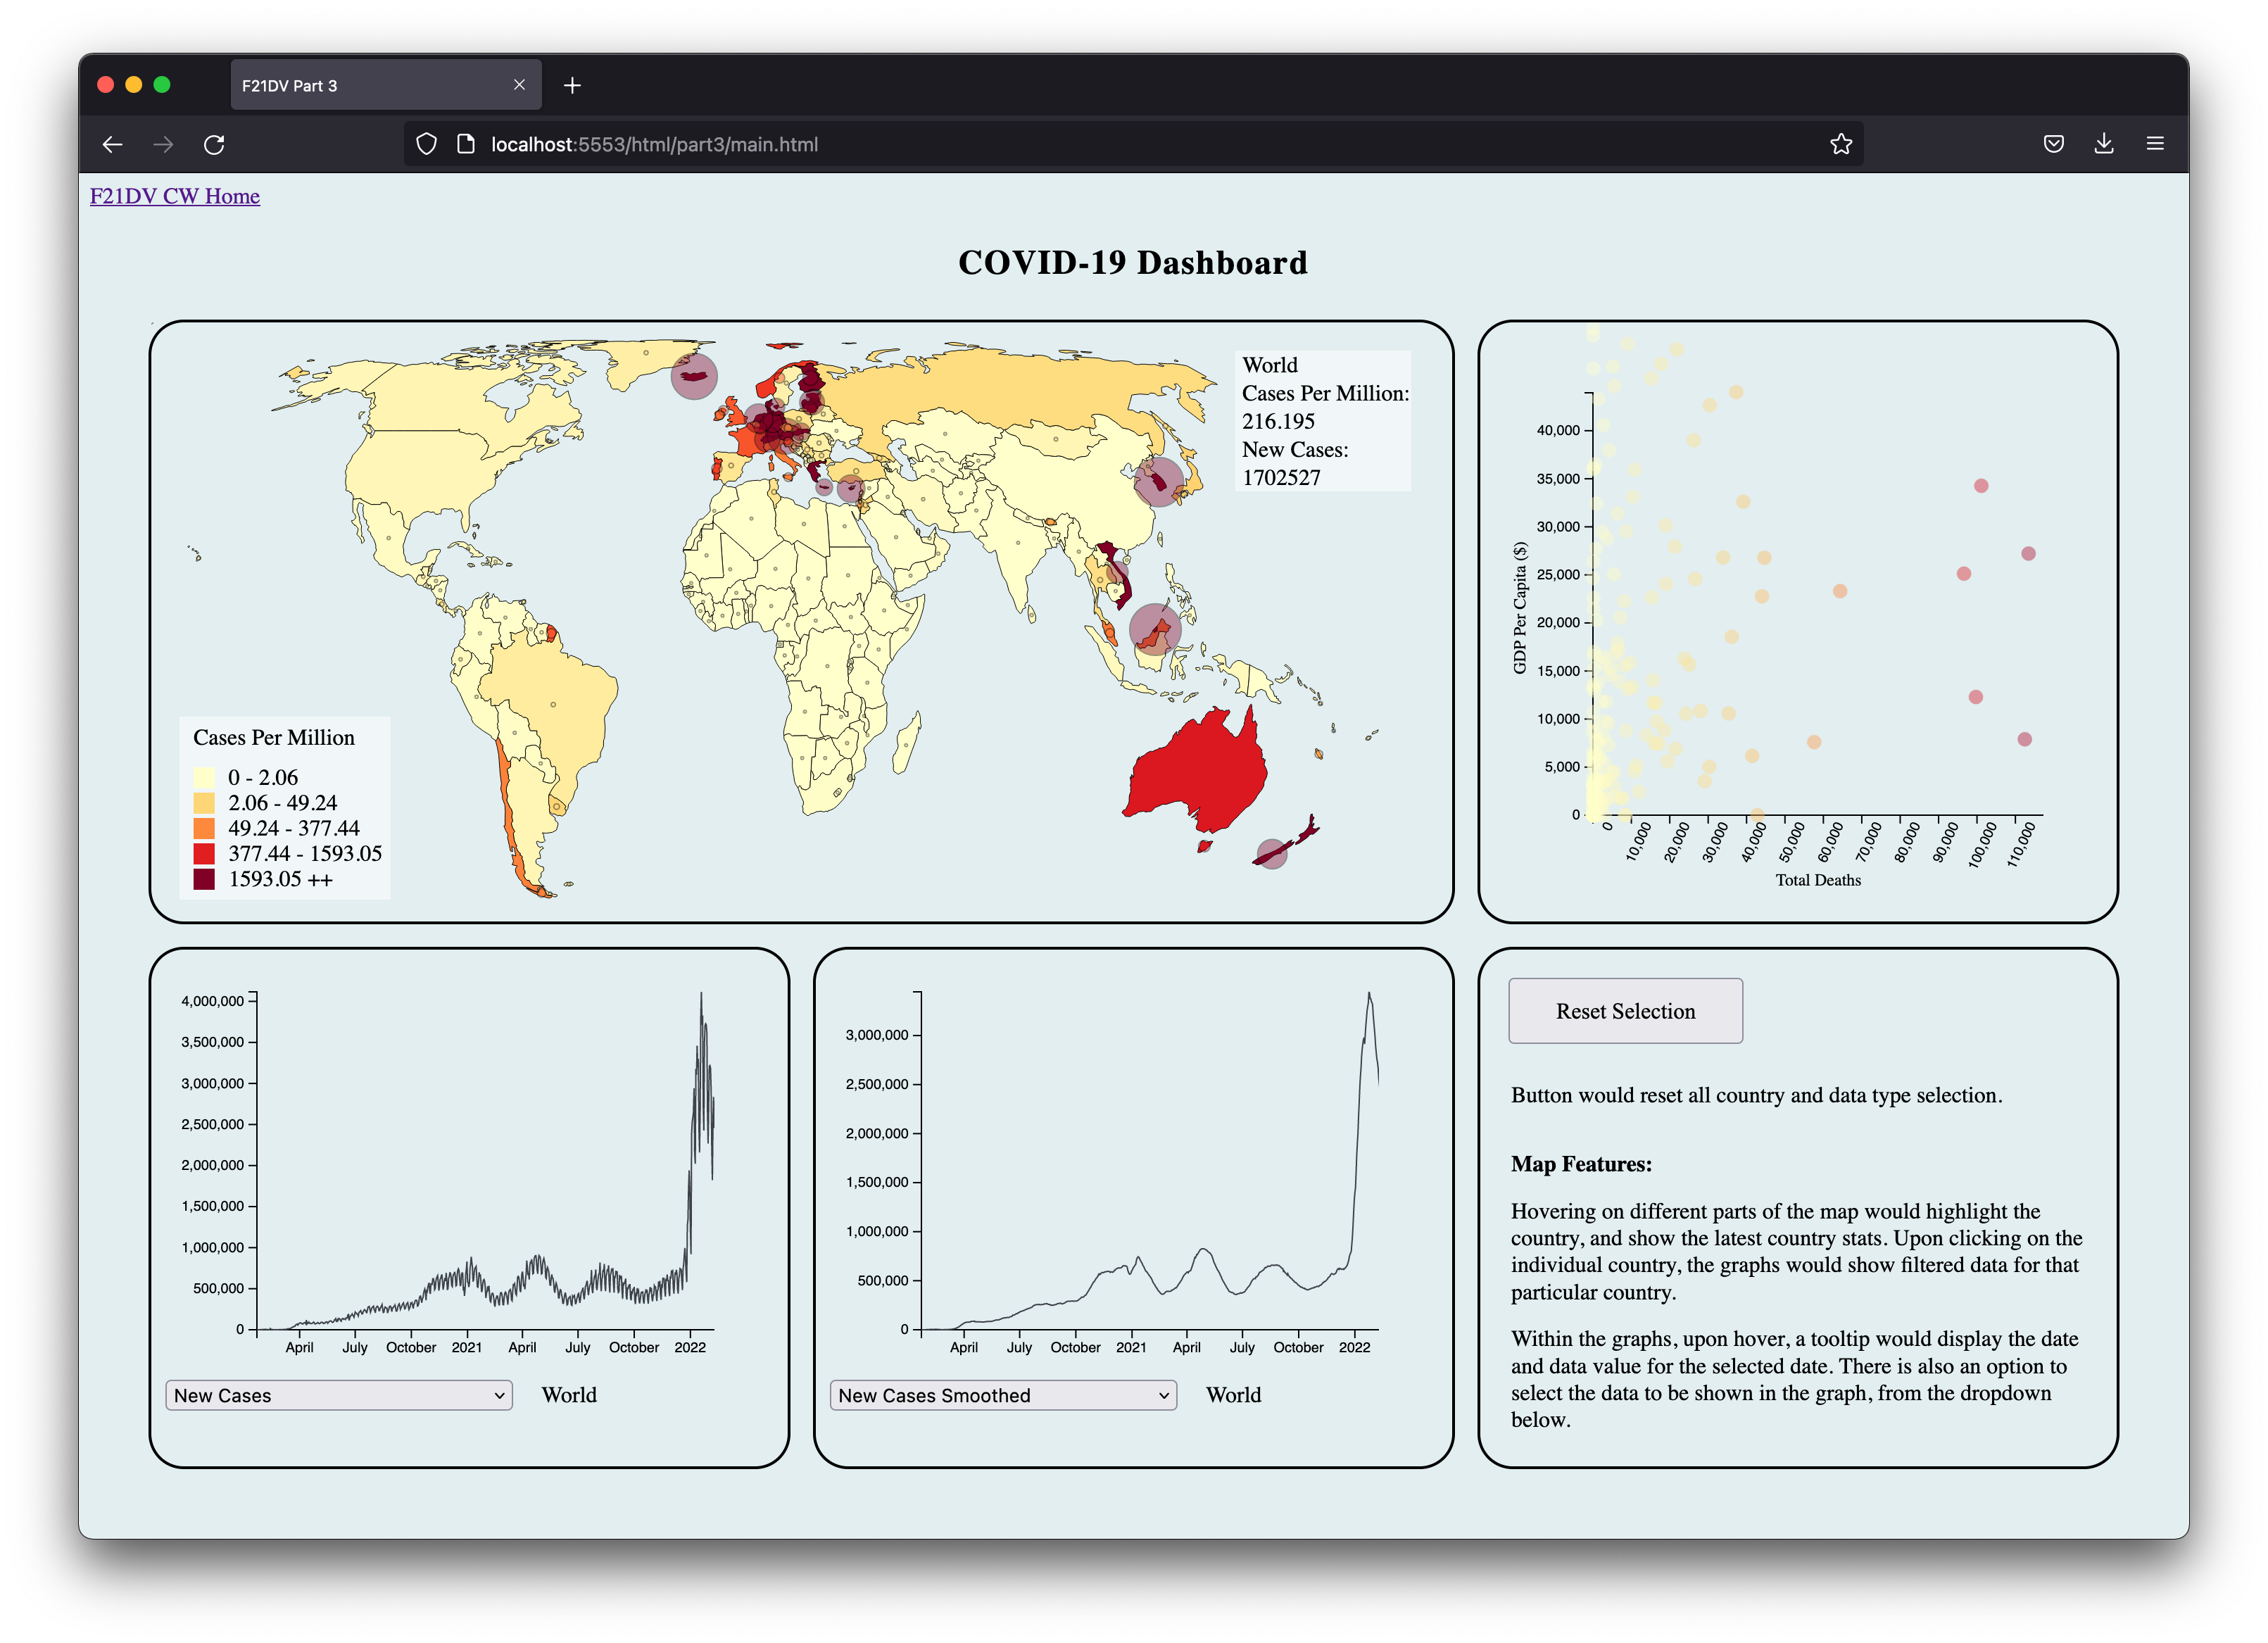
\includegraphics[width=\textwidth]{images/main.png}
    \caption{Full Dashboard View}
    \label{fig:main}
\end{figure}
Shown in figure \ref{fig:main} is the main view of the Covid-19 Dashboard, made out of a few different layouts namely the map, the line graphs below, and a scatter plot. 

\newpage
\section{The Map}
\begin{figure}[H]
    \centering
    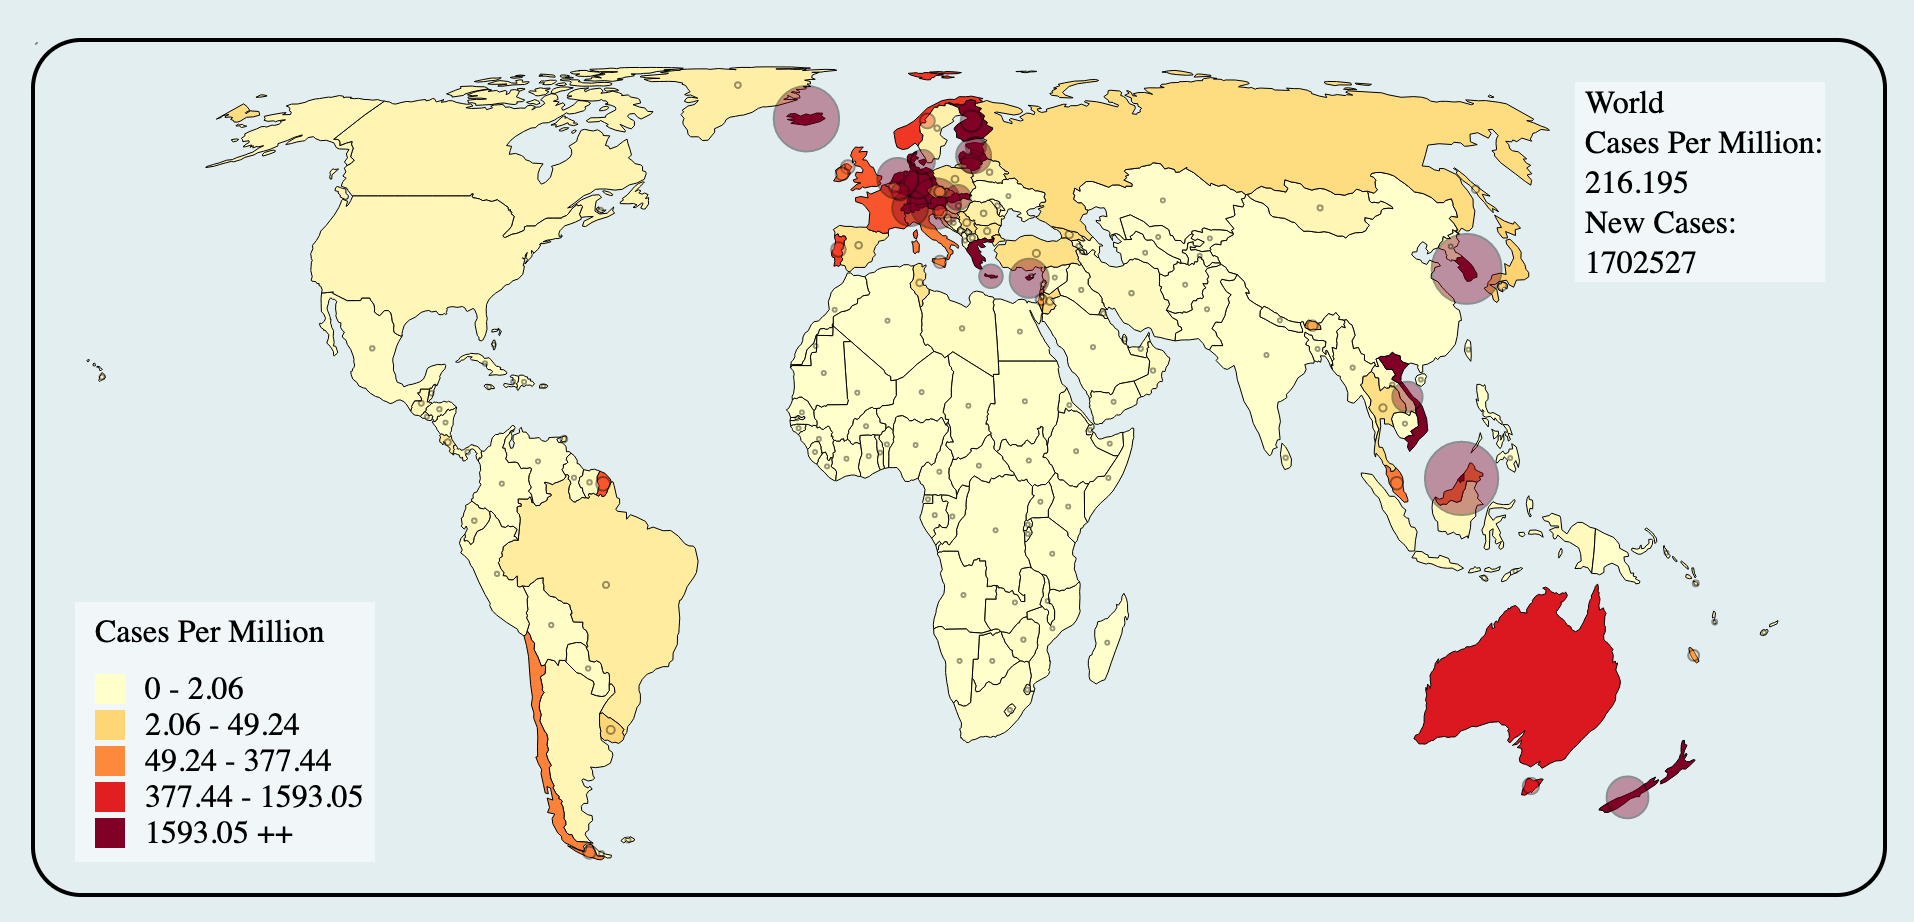
\includegraphics[width=\textwidth]{images/map.png}
    \caption{Closeup View of Map}
    \label{fig:map}
\end{figure}
A closeup view of the map, as shown in figure \ref{fig:map}, would show a colour coded map based on the latest \textbf{New Cases Per Million} Covid-19 numbers, as well as circles indication where the covid hotspots all over the world are. The map also containes a legend on the top right showing a country's latest cases numbers upon mouse hover (World's data if mouse is not on any country).

The map container is first filled with an svg. Then the rest of the elements are just shapes and objects that were later on added onto the svg. 
\vspace{8pt}
\lstinputlisting[firstline = 83, lastline = 90, label = {lst:map-projection}, caption = {Map Projection}]{../../public/js/part3/main.js}
From listing \ref{lst:map-projection}, we could see the projection that was used to scale the geojson polygons and add them to the map. I have chosen the \verb|.geoEqualEarth()| scaling method since it is the best way to see the size of different countries in relation to one another. This would be the best choice for viewing covid data, as we could now see how big and small countries react to covid-19 differently. 
\vspace{8pt}
\lstinputlisting[firstline = 172, lastline = 199, label = {lst:plot-map}, caption = {Adding the Map}]{../../public/js/part3/main.js}
Listing \ref{lst:plot-map} shows the how the map is added to the svg. \verb|topo[0].features| is the geojson file that was passed into the d3 function. An abstract of it can be seen in appendix section \ref{ap:geojson}. Using \verb|d3.geopath()|, the map could be added onto the svg, country by country, and the fill of each country | the colour coded case numbers of each country is added on using the function in line 9 to 20.
\par The function first takes the data, \verb|d| value for each country and obtain its id, \verb|d.id|, then uses a default JavsScript array function \verb|.find()| to obtains the latest case numbers from the \verb|dataCase| array, which stores the latest case numbers for all the countries. Then, a function that checks for null value is in place to ensure that even if a country does not have any numbers, they could still have a colour. Lastly, the case numbers are passed into the colour scale function to return a colour value. The same thing is also for the circles, just that there is also a function that sizes the circles according to the case numbers.

\subsection{Map on Mouse Over}
\begin{figure}[H]
    \centering
    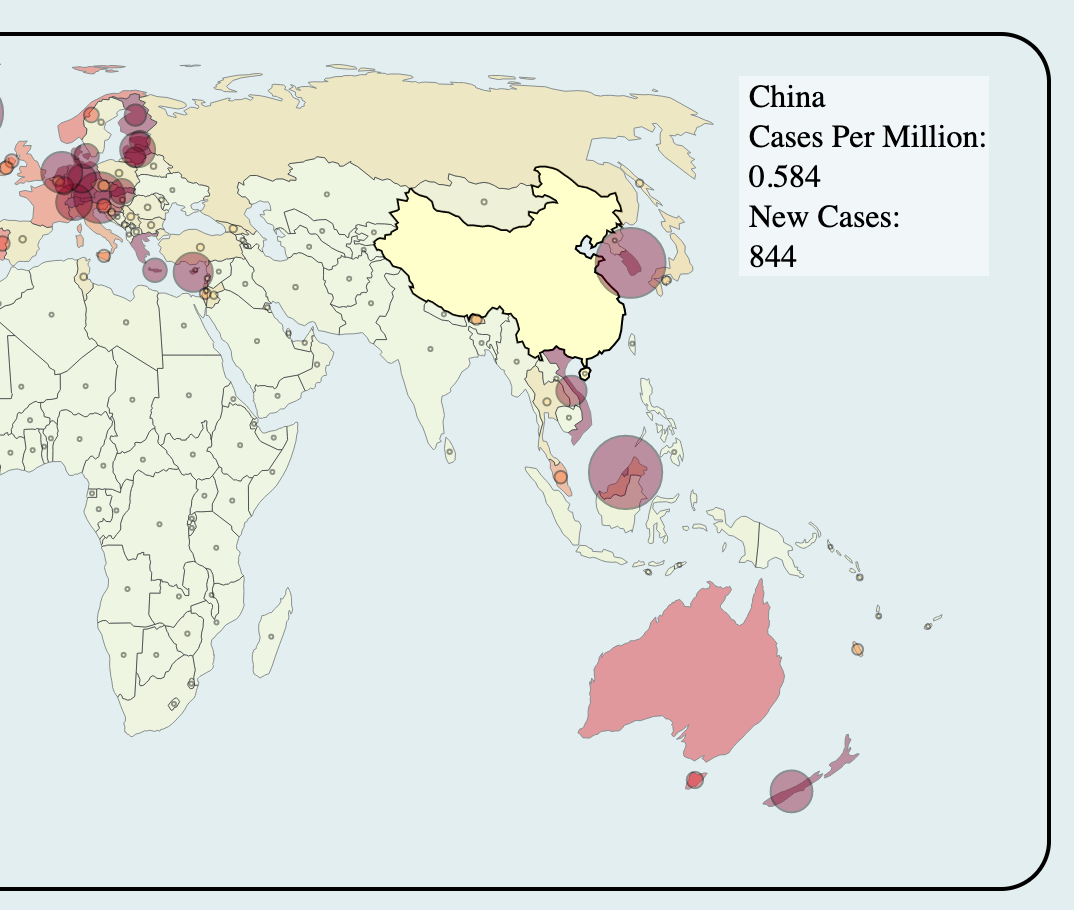
\includegraphics[width=0.4\textwidth]{images/hover-map.png}
    \caption{Map on Mouse Hover}
    \label{fig:map-hover}
\end{figure}
Figure \ref{fig:map-hover} shows what happens to the map on mouse over action. Upon mouse over, on any country, the map's upper right tooltip would show the country's name, cases per million, as well as the latest new cases numbers. 
\vspace{8pt}
\lstinputlisting[firstline = 92, lastline = 120, label = {lst:map-mouseover}, caption = {Map's Mouse Over Function}]{../../public/js/part3/main.js}
Figure \ref{lst:map-mouseover} shows how the mouseover function is achieved. On mouseover, d3 parses the data through the function, and once again, using the native \verb|.find()| function for JavaScript arrays, we find the data for said country, and using that, we rename the tooltip using a \verb|d3.select()| and \verb|.text()| function. The function also highlights the selected country, and increases its stroke width so that it is more obvious in highlight. 

In this case, since the latest data is on the 14th of March, china has 0.584 cases per million people, and have 844 new cases on that day.

\subsection{Map on Mouse Click}
\begin{figure}[H]
    \centering
    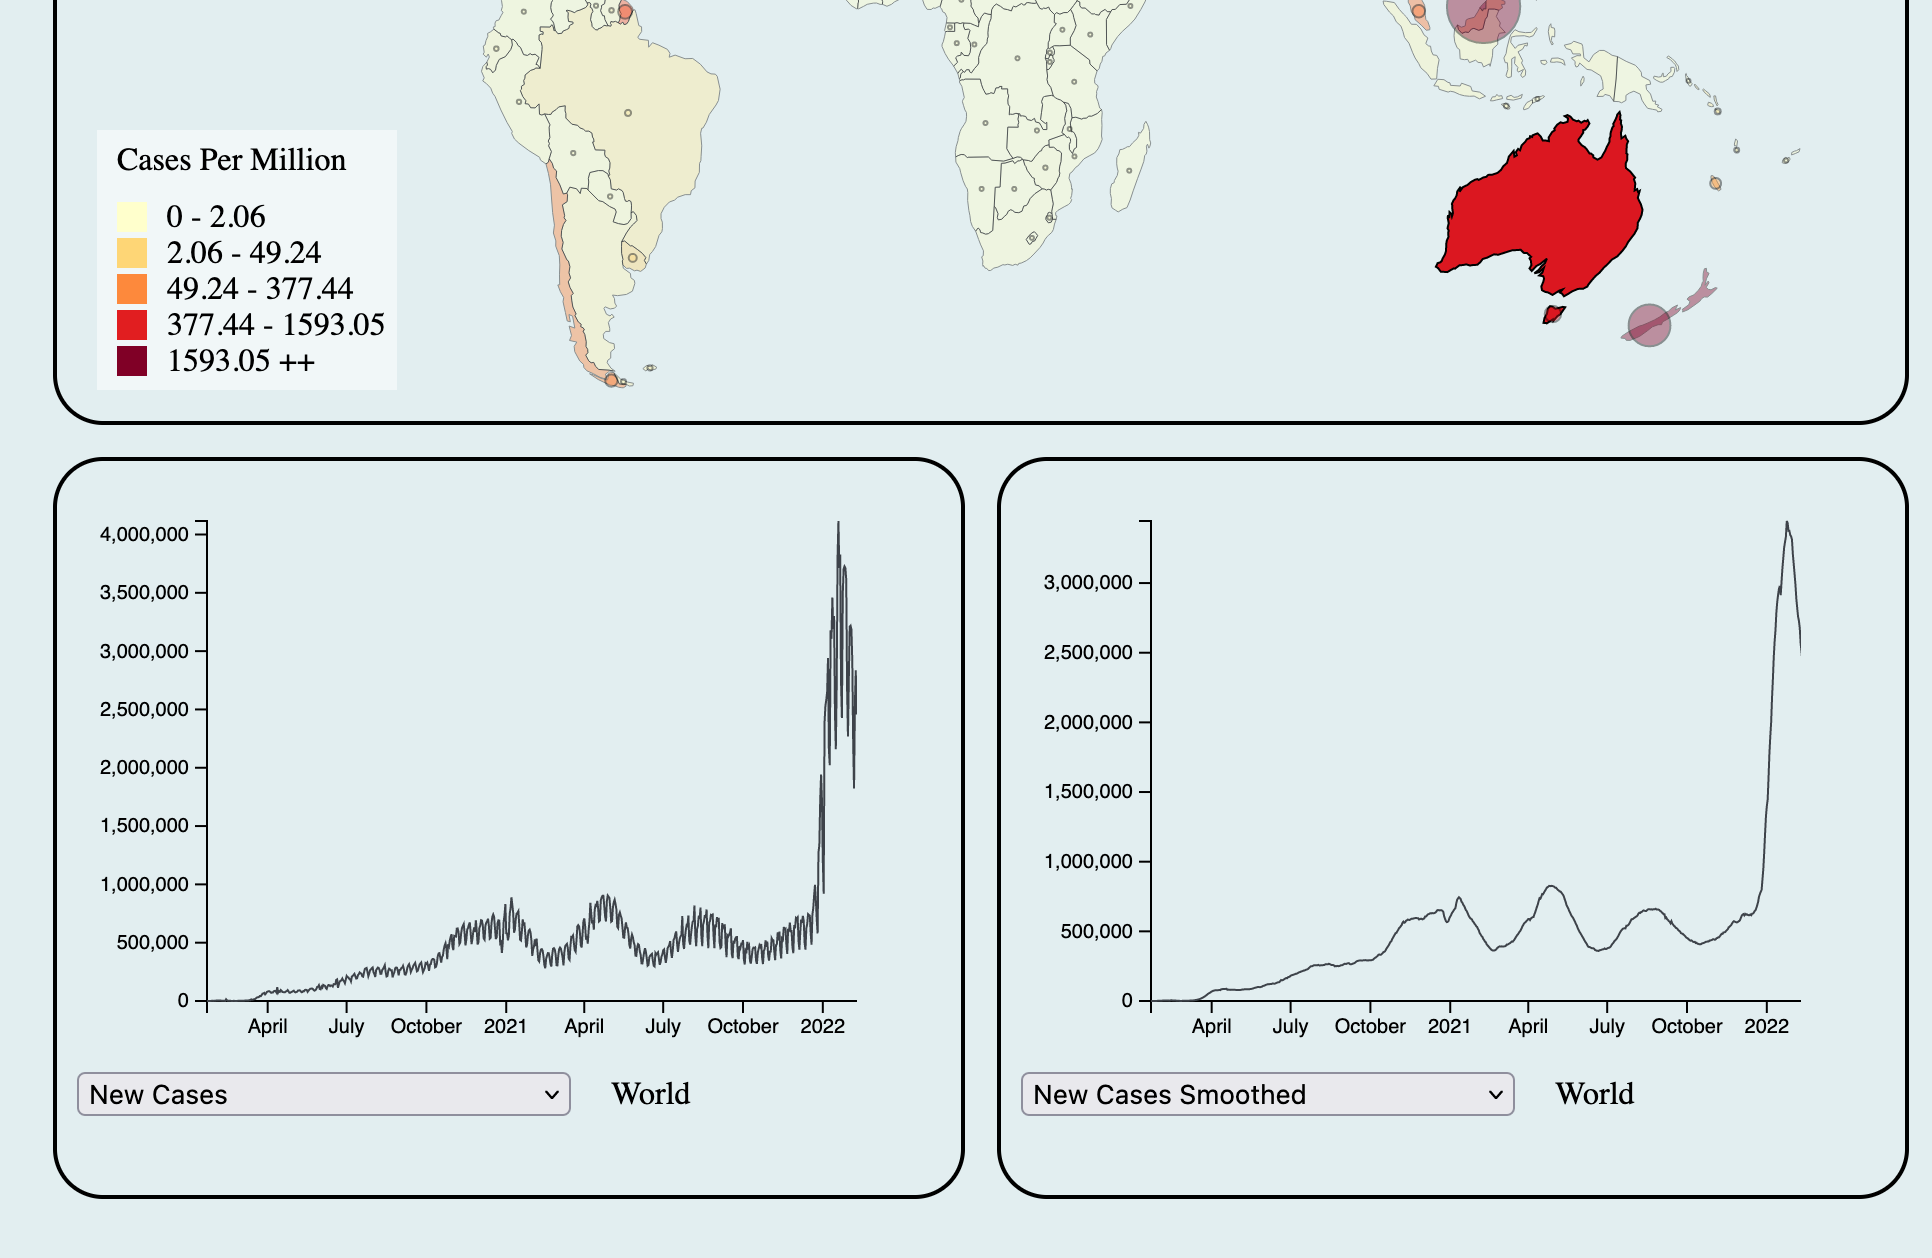
\includegraphics[height=0.3\textwidth]{images/click_1.png}
    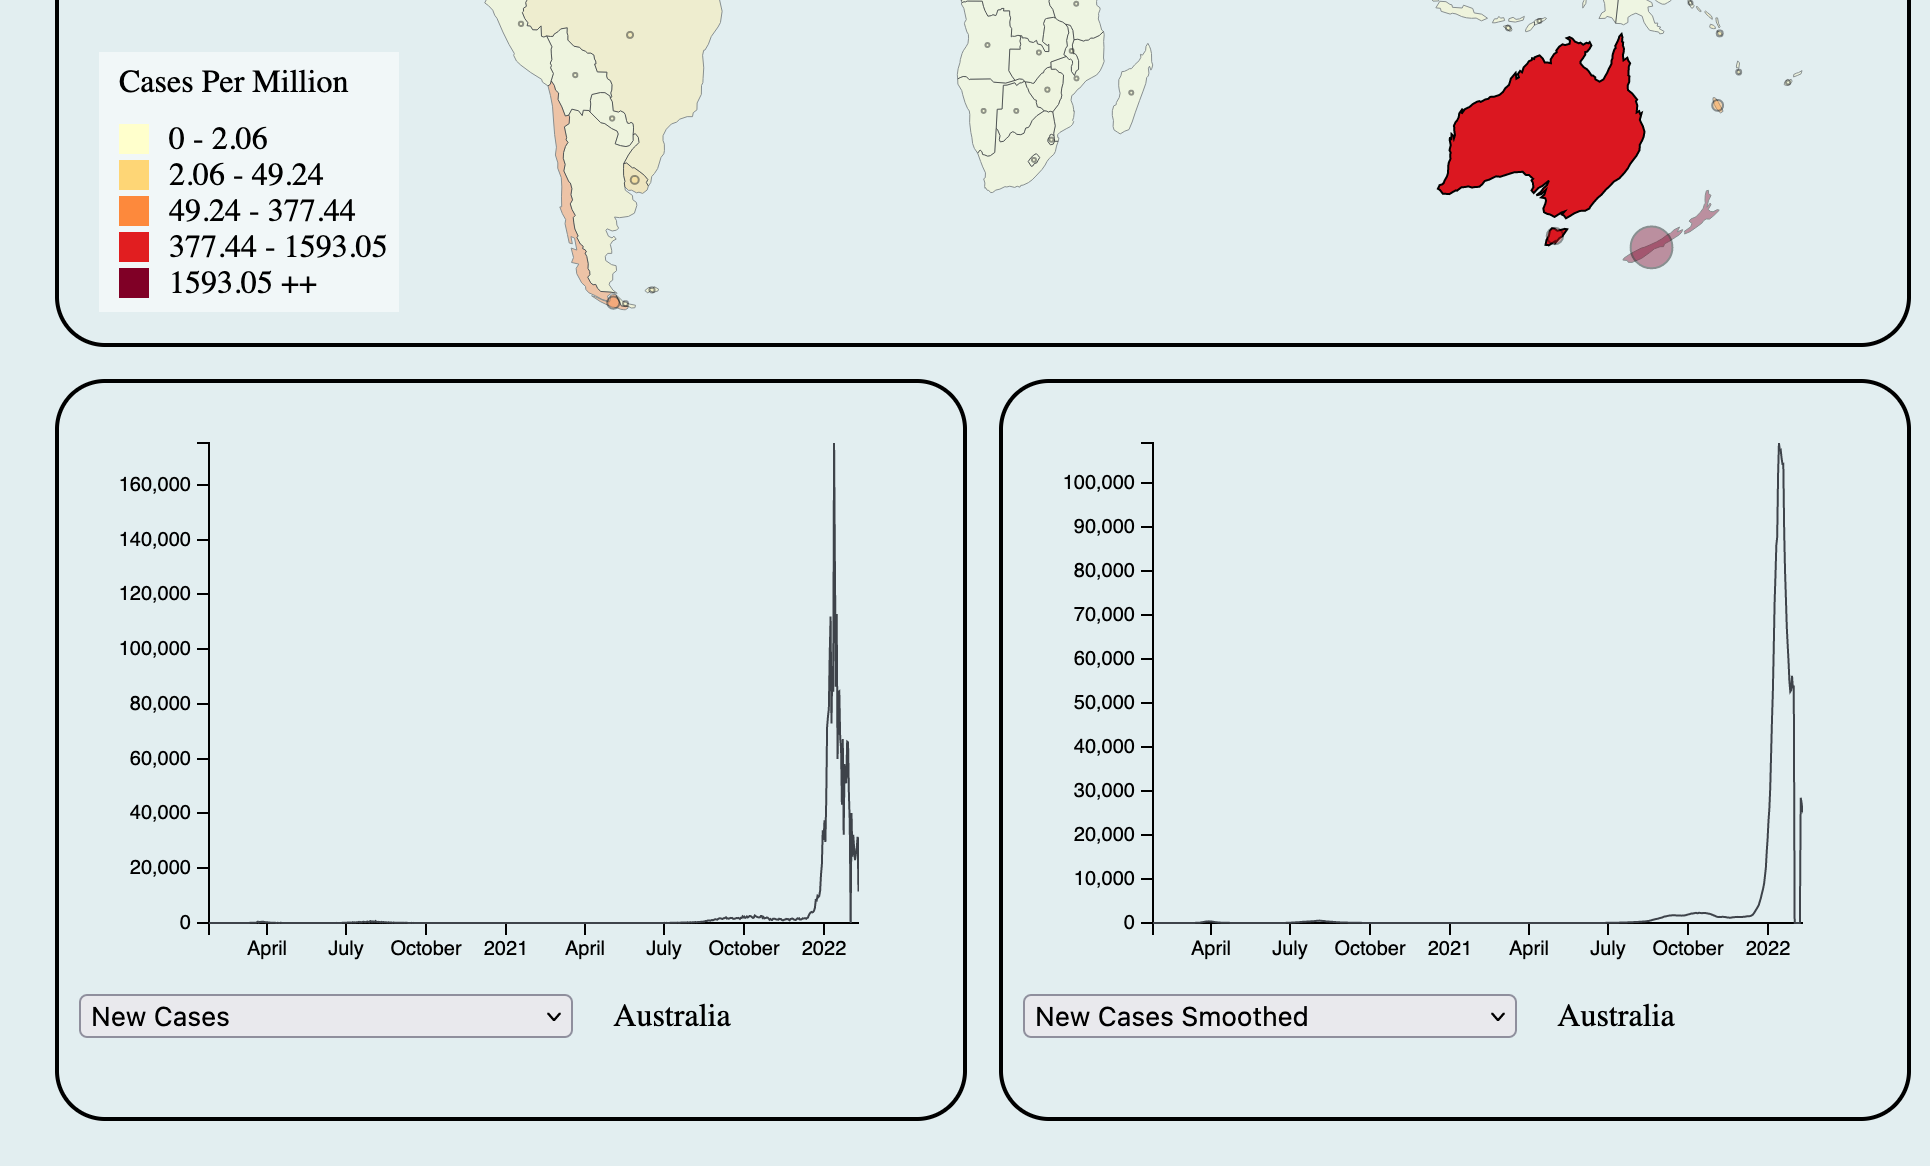
\includegraphics[height=0.3\textwidth]{images/click_2.png}
    \caption{Map on Mouse Click}
    \label{fig:map-click}
\end{figure}
Figure \ref{fig:map-click} shows the before and after of clicking on \textbf{Australia} in the map. Upon clicking, the graph section below would be updated with the Australian case numbers, by default, it would be New Cases and New Cases Smoothed. The x and y axis would be updated too. The detailed update mehtod of the graph would be further dicussed later.
\vspace{8pt}
\lstinputlisting[firstline = 146, lastline = 170, label = {lst:map-click}, caption = {Map's Mouse Click Function}]{../../public/js/part3/main.js}
Listing \ref{lst:map-click} shows the click function processing the mosuse click event on the map. Upon click, the mouse would obtain the country's data using a predefined function \verb|getCountryData()| which returns an array of all the country's data. Using the same array, and the native \verb|.find()| function, we then obtain the country's name. Then using the \verb|updateGraph()| function, the graphs are now both updated. If the array containes no data, there would also be a no data sign that is shown beside the country name. 

\section{The Graph}
\lstinputlisting[firstline = 24, lastline = 31, label = {lst:graph-scale}, caption = {Graph Axes Scale}]{../../public/js/part3/graph.js}
\lstinputlisting[firstline = 41, lastline = 51, label = {lst:graph-plot}, caption = {Plotting the Graph}]{../../public/js/part3/graph.js}
Listing \ref{lst:graph-scale} shows the scale method used for the X and Y axes of the graph. Using these scales, later then in \ref{lst:graph-plot}, they were used to define the line for the graphs. Finally, to draw the base of the graph, these scales and lines were used to draw the base graph, before calling an update function. 

\subsection{The updateGraph() function}
The function takes on \verb|dataUpdate|, \verb|type| and \verb|selector| as parameters, where \verb|dataUpdate| is the newest data | to be used with upon click of a country, \verb|type| to be used with selecting the dropdown menu on the graph, and finally the \verb|selector| to differentiate the use of said function of the different graph. 

Upon update, the graphs do many things. Amongst which are replotting the graph, and renaming the country selected. 

\subsubsection{Updating the Graph Line}
\lstinputlisting[firstline = 100, lastline = 131, label = {lst:graph-replot}, caption = {Updating the Graph}]{../../public/js/part3/graph.js}
Listing \ref{lst:graph-replot} shows the code that was used to update the line graph. First, using the new data, \verb|dataUpdate|, a new x and y axis scale was obtained, and then re-added onto the graph. A transition was also used, to smoothly add the axis. 

Later, on line 22 onwards, a new line is defined, and then recalled onto the existing line using a transition. 

\subsubsection{Adding a Tooltip}
\begin{figure}[H]
    \centering
    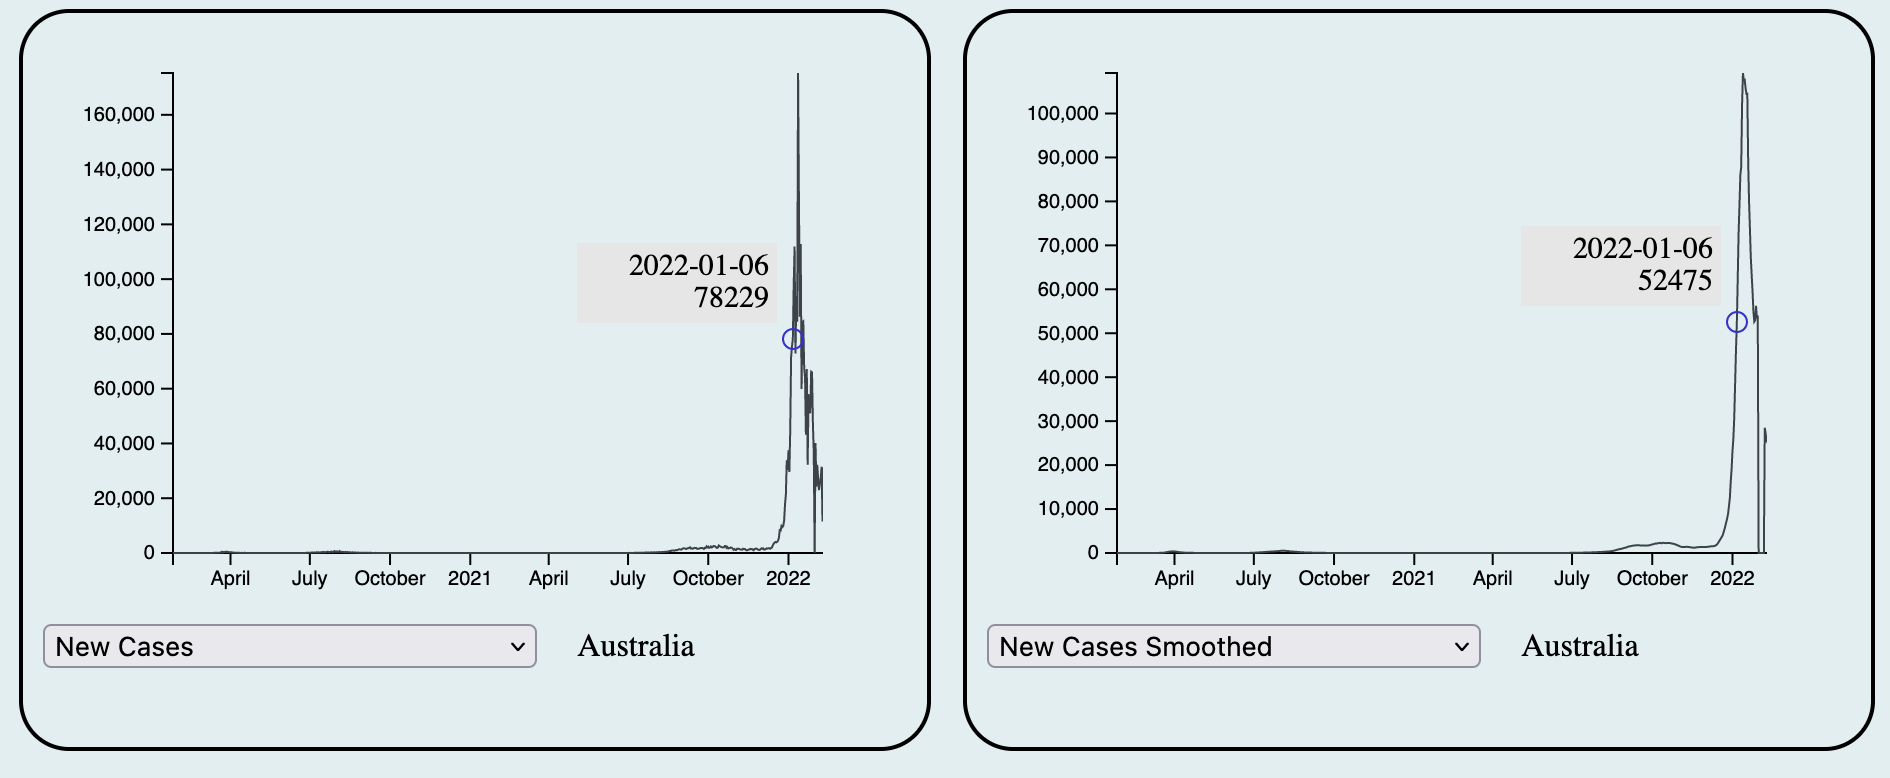
\includegraphics[width=\textwidth]{images/graph-tooltip.png}
    \caption{Map on Mouse Click}
    \label{fig:graph-tooltip}
\end{figure}
Figure \ref{fig:graph-tooltip} shows a tooltip appearing on hover of the line graph. Due to the length of the code, the code could be viewed \href{https://github.com/jonleesy/F21DV-Coursework/blob/main/public/js/part3/graph.js}{here}.The idea is that both graphs would sahre the same x-axis value, hence the same point on the x-axis. The only difference is the different `type' of data. Hence, there was two difference type of y scale, hence a different translation of the y axis for both the graphs. 

\subsection{The Dropdown Selector}
\begin{figure}[H]
    \centering
    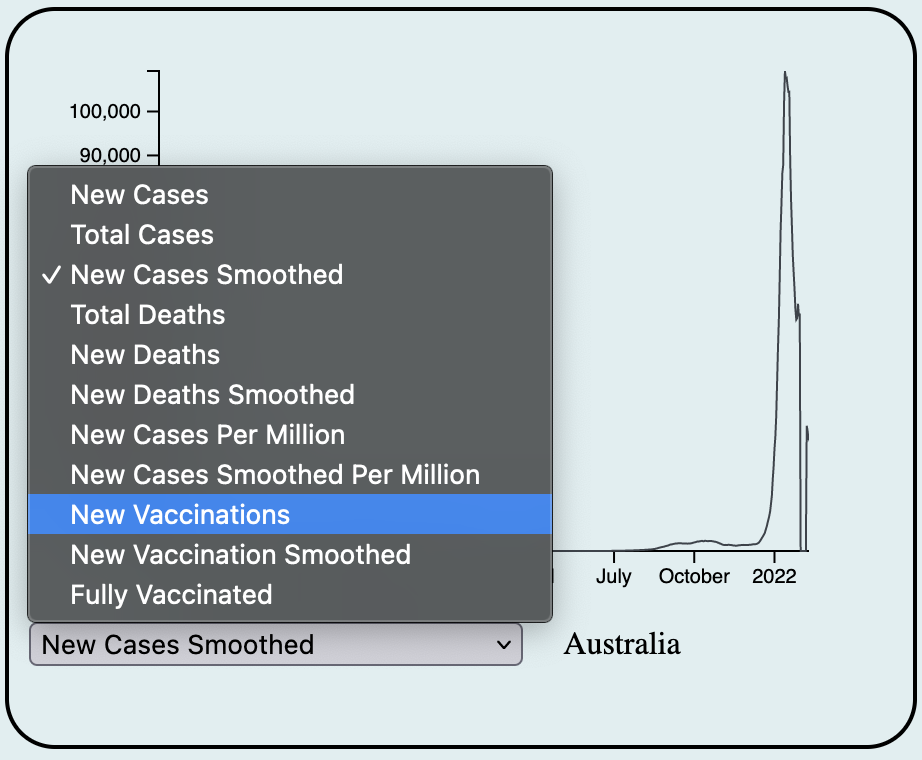
\includegraphics[height=0.3\textwidth]{images/selector_1.png}
    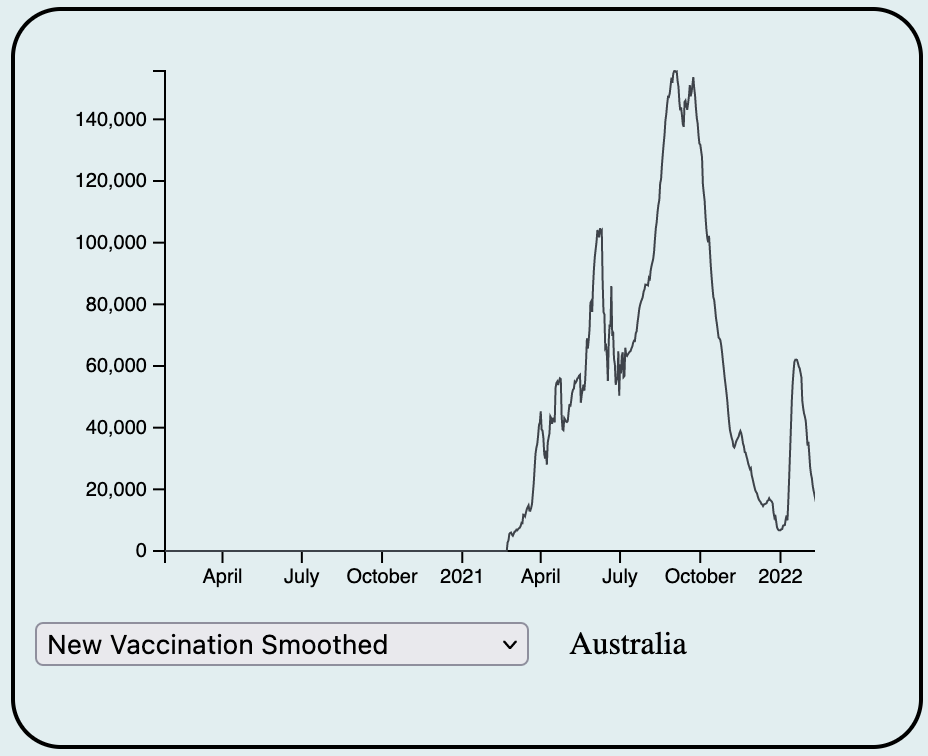
\includegraphics[height=0.3\textwidth]{images/selector_2.png}
    \caption{Graph Selector}
    \label{fig:graph-selector}
\end{figure}
Figure \ref{fig:graph-selector} shows the dropdown selector for each individual graph. From the figure shown, we could see that upon select, the graph would be updated with a new data. This would use the \verb|updateGraph()| function as well, and updating the `type' parameter.

\section{The Scatter Plot}
The scatter plot is just a simple case of adding circles to the svg. This is by using the latest New Deaths data, and the newest GDP per capital data to determin a circle's X and Y axis. The circle is then colour-coded using the same colour scale for the map. 

\section{The reset button}
The reset button does 2 things:
\begin{itemize}
    \item Resets the graph selection to world's data.
    \item Resers individual graph's data to default: New Cases and New Cases Smoothed.
\end{itemize}

\newpage
\chapter{Queries}
\section{Is there a relation between the relative ‘wealth’ of a population and the evolution of the pandemic?}
We could see from the scatter plot, that there is a cluster of low GDP Per Capita countries with low deaths, this is at the lower left of the graph. The rest of the countries are just scattered around the graph. This does not show anything about the relation between wealth and population. This just shows that there are just more countries with a low GDP, hence also a higher percentage of countries with low death rates. 

\section{What is the effect of vaccinations on the spread of cases/deaths and display any effect (if any) that booster jabs have on the cases/deaths.}
\begin{figure}[H]
    \centering
    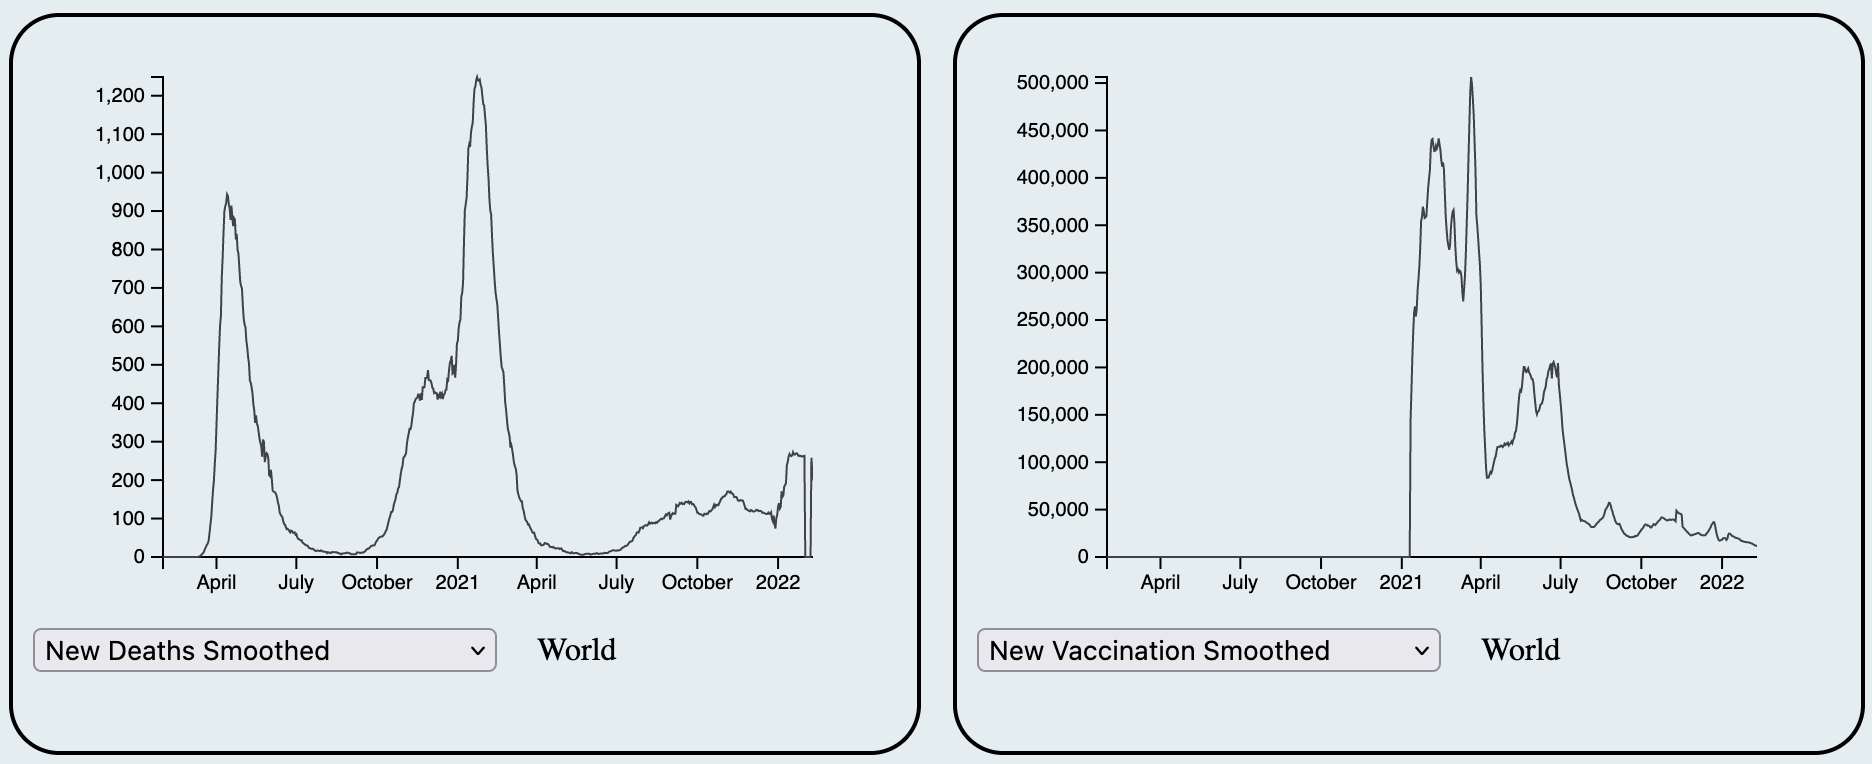
\includegraphics[height=0.3\textwidth]{images/death-vacc.png}
    \caption{Vaccinations on death}
    \label{fig:vacc-death}
\end{figure}
Figure \ref{fig:vacc-death} shows the effect of vaccinations on the death rates. As we could see, as people started getting vaccinated, the peaking death rates started to come back down as well. To know if there is a full effect of vaccinations on the death rates, there needs to be some coorelation analysis on these two data. 


\newpage
\chapter{Appendices}
\section{GeoJson File}
\lstinputlisting[firstline = 10, lastline = 20, label = {ap:geojson}, caption = {GeoJson Abstract}]{../../public/data/part3/geojson.json}

\end{document}